Nous avons fait le choix d'utiliser un framework nommé Laravel. Ce framework est assez récent et a pour objectif de faciliter le développement. Son slogan est \enquote{\textit{PHP that doesn't hurt. Code happy and enjoy the fresh air."}}. Depuis l'année 2013 Laravel a connu un succès important et il est depuis peu le framework PHP attirant le plus de recherches comme montré dans la figure \ref{fig:trends-php-frameworks}.

\begin{figure}[H]
	\centering
	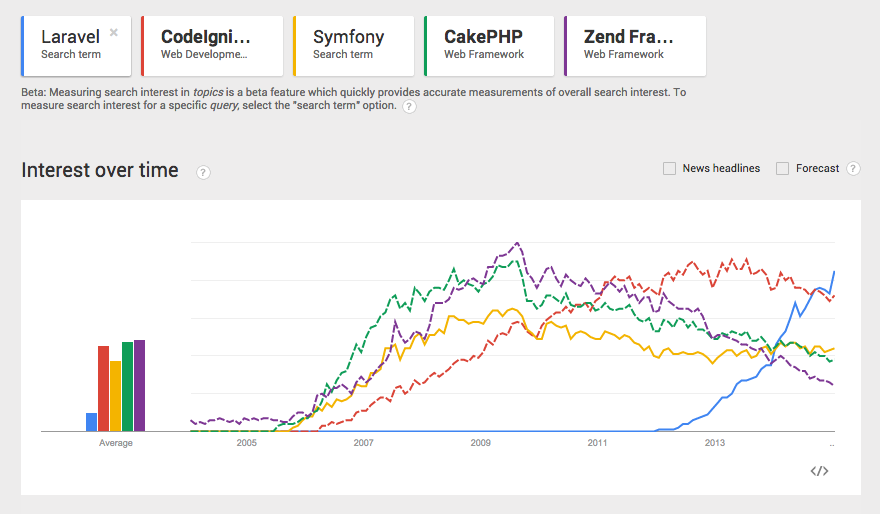
\includegraphics[width=1\textwidth]{images/trends-php-frameworks.png}
	\caption{Recherches Google pour les principaux frameworks PHP.}
	\label{fig:trends-php-frameworks}
\end{figure}

\section{Un framework MVC}
	Laravel est un framework mettant en avant une séparation très importante des modèles, des vues et des contrôleurs. Toutes les classes que nous avons créé se trouvent dans le dossier \verb|app/Insa| et sous l'espace de nom (\textit{namespace}) \verb|Insa|.\\

	Nous avons choisi une architecture modulaire organisée selon les entités. À chaque entité on associe les dossiers suivants :
	\begin{itemize}
		\item \verb|Controllers| : les contrôleurs associés à l'entité ;
		\item \verb|Models| : les modèles associés à l'entité. Généralement il n'y a qu'une classe dans ce dossier qui correspond au singulier de l'entité, par exemple \verb|\Insa\Recipes\Models\Recipe| ;
		\item \verb|Presenters| : les classes qui ont pour objectif d'effectuer les transformations nécessaires afin de présenter les données brutes dans l'application web ;
		\item \verb|Repositories| : les classes d'accès aux bases de données ;
		\item \verb|Validation| : les classes comportant les règles de validation des entités.
	\end{itemize}

\section{Les \servicesProvider{}}
	Les \servicesProvider{} sont le centre de Laravel. Ce sont des classes qui permettent de lier des objets entre eux et d'enregistrer des éléments de configuration. Ce sont dans ces classes que l'on retrouve par exemple la liaison entre les routes et les méthodes des contrôleurs : ce qui permet qu'une méthode soit appelée en fonction de l'URL.\\

	Les \servicesProvider{} se trouvent à la racine de chaque espace de nom. Nous avons défini la convention suivante pour les noms de ces classes : \verb|\Insa\<entite>\<entite>ServiceProvider|. Un \serviceProvider{} minimal, définissant une URL en tant que route gérée par un contrôleur, est présenté dans le listing \ref{code:service-provider-minimal}.
	\begin{listing}[H]
		\inputminted{php}{code/serviceProvider.php}
		\caption{Un exemple de \serviceProvider{} liant la page d'accueil à une liste de toutes les recettes.}
		\label{code:service-provider-minimal}
	\end{listing}

\section{Injection de dépendance et \ioc{}}
\label{sec:ioc}
	Il est très rare d'instancier des classes lorsque l'on utilise Laravel. Tout d'abord, on peut remarquer que quand on enregistre des routes, on donne le nom du contrôleur, et non une instance de celui-ci. Laravel se charge de l'instanciation de la classe à notre place lorsque la route enregistrée est demandée. Pour instancier une classe, Laravel utilise un outil très puissant de résolution de dépendance se basant l'introspection de PHP. Avant de créer l'objet nécessaire, elle détermine les classes requises par le constructeur et les injecte. La résolution de dépendance est faites de manière récursive.\\

	En plus de la résolution automatique de dépendance, Laravel utilise l'\ioc{}. L'\ioc{} est un entrepôt de classes permettant de lier une interface à une implémentation concrète, où une chaîne de caractères à une classe par exemple. Cette dernière possibilité est présentée dans le listing \ref{code:ioc-container}.

	\begin{listing}[H]
		\inputminted{php}{code/iocContainer.php}
		\caption{Un exemple d'utilisation de l'\ioc{}.}
		\label{code:ioc-container}
	\end{listing}

	Si le constructeur d'un contrôleur nécessite par exemple un objet \verb|Insa\Recipes\Repositories\RecipeRepository|, Laravel va utiliser l'injection de dépendance et l'\ioc{} afin de lui fournir une implémentation concrète qui aura été associée à l'interface. Cet exemple est présenté dans le listing \ref{code:ioc-controler}.
	\begin{listing}[H]
		\inputminted{php}{code/injectionClass.php}
		\caption{Injection d'une interface dans un constructeur de contrôleur.}
		\label{code:ioc-controler}
	\end{listing}

	De cette manière, nous avons accès au répertoire dans notre contrôleur sans effort.

\section{Les façades}
	Une façade est un classe spécifique qui permet d'appeler des méthodes publiques d'une instance d'un objet via des appels statiques sur la façade. Les classes qui peuvent être résolues par des façades sont celles qui se trouvent dans l'\ioc{} (abordé dans la partie \ref{sec:ioc}).\\

	Par exemple, lorsque que l'on appelle une méthode statique sur la façade \verb|Route|, Laravel va en réalité appeler une méthode publique d'une instance d'une classe appelée \verb|Illuminate\Routing\Router| stockée dans l'application.\\

	On se retrouve alors avec deux possibilités dans les contrôleurs :
	\begin{itemize}
		\item utiliser des appels statiques via les façades ;
		\item injecter les véritables classes dans le constructeur et appeler des méthodes sur cette classe via un attribut de classe.
	\end{itemize}
	\vspace{10px}
	La deuxième option est généralement préférée, étant réputée plus propre. Pour autant l'utilisation des façades n'est pas totalement à proscrire.

\section{Le \repositoryPattern}

	\subsection{Description}
		Le \repositoryPattern{} est une bonne pratique de modélisation permettant d'abstraire la manipulation des données. Les objectifs sont nombreux :
		\begin{itemize}
			\item Uniformiser l’interaction avec les données à travers l'application ;
			\item Séparer la logique métier de l'accès aux données ;
			\item Faciliter les tests d'intégration en isolant la couche d'accès aux données ;
			\item Proposer plusieurs moyens d'accès aux données (bases de données, cache, fichiers, API\dots), tout en uniformisant les méthodes à l'aide d'interfaces.
		\end{itemize}

	\subsection{Pourquoi utiliser des répertoires}
		Dans le cas d'une application plutôt simple comme la notre, il aurait été parfaitement correct d'appeler les méthodes de l'ORM\footnote{ORM : \textit{Object Relational Mapper.}} de Laravel, Eloquent, directement dans les contrôleurs.\\

		Mais dans le cas d'une application plus complexe, il est préférable de dissocier ses contrôleurs de l'ORM afin d'améliorer la maintenabilité de l'application et de permettre l'utilisation d'un autre système de stockage. En effet, si l'on décidait de passer à une autre méthode de stockage que celle choisie initialement, il faudrait aller chercher dans toute l'application où sont effectués ces accès. En utilisant le \repositoryPattern{} il suffit de créer une nouvelle classe respectant le contrat initial (l'interface créée) puis vérifier que celle-ci est conforme aux test écrits.

	\subsection{Utilisation de répertoires}
		La création de répertoires est finalement assez simple. Les différentes étapes sont le suivantes :
		\begin{enumerate}
			\item Création d'une interface indiquant le comportement attendu pour l'accès aux données ;
			\item Création d'une classe concrète se conformant à l'interface en utilisant l'ORM de Laravel ;
			\item Association de l'interface à la classe concrète créée dans un \serviceProvider.
		\end{enumerate}

		Un exemple d'interface d'accès aux données concernant les recettes est présenté dans le listing \ref{code:recipes-repo-interface}. Son implémentation concrète est présentée dans le listing \ref{code:recipes-repo-mongo}.

		\begin{listing}[H]
			\inputminted{php}{code/RecipesRepository.php}
			\caption{L'interface spécifiant le contrat d'accès aux données des recettes.}
			\label{code:recipes-repo-interface}
		\end{listing}

		\begin{code}
			\inputminted{php}{code/MongoRecipesRepository.php}
			\caption{Utilisation de l'ORM Eloquent pour l'accès aux données des recettes.}
			\label{code:recipes-repo-mongo}
		\end{code}